\documentclass[a4paper,12pt]{article}

\usepackage{amsmath,amssymb,amsthm,tikz}
\usetikzlibrary{calc,arrows.meta}
\usepackage[margin=20mm]{geometry}
\usepackage{fancyvrb}
\usepackage{enumerate}
\usepackage{hyperref}

\setlength{\parindent}{0pt}
\setlength{\columnsep}{1cm}

\newcommand{\indsize}{\scriptsize}
\newcommand{\colind}[2]{\displaystyle\smash{\mathop{#1}^{\raisebox{.5\normalbaselineskip}{\indsize #2}}}}
\newcommand{\rowind}[1]{\mbox{\indsize #1}}

\begin{document}
\thispagestyle{empty}

\twocolumn

\begin{center}
{\Large Sample Final. 2020-12-16.}\\
{\em This sample (unlike the actual exam) 
is NOT scaled to fit in 120 minutes.} 
\end{center}

{\footnotesize 
{\bf Summary.} This is a sample exam, it only gives an 
approximate idea regarding the question types and their difficulty. 
The actual exam may cover some other topics (it may also include 
things taught before the midterm exam). 

Final exam emphasizes certain things that are important for further
IT subjects (such as Time Complexity, Graph Algorithms) and also 
the knowledge used in practical programming 
(using standard libraries and ensuring integrity of data structures
and their representation invariants).
}


% 
\vspace{10pt}
{\bf Question 1 (Time Complexity).} 
% BubbleSort + custom comparison


\vspace{5pt}
{\bf (A)} We need a sorting algorithm that would order all pairs of integers $(x,y)$ 
by the first number $x$ (and by the second number $y$, if the first 
numbers in the pair are equal). For example $(1,100) < (2,10) < (2,20) < \ldots$. 
Which comparison function can be passed as a parameter to 
the sorting method ${\tt sort(...)}$ on Line 38.

\vspace{5pt}
{\bf (B)} As we know, we can define various ways how compare 
objects.
%(we can order pairs by their sum $x+y$, or by their product $x \cdot y$, 
%or first order by the second number $y$ in decreasing order, 
%then by the first number $x$ in increasing order, and so on).\\
Are there any mathematical properties that a comparison algorithm $\mathtt{Comp(...)}$ 
should satisfy to be passed as a parameter to a sorting algorithm like the one above? 
(Please list just the most general properties that 
do not depend on the object types to be sorted and the
particular ordering that you need.)

 
\vspace{5pt}
{\bf (C)} What is the time complexity of the sorting algorithm 
shown on Line 18--32 of the code? Express your answer as $O(g(n))$,
where $n$ is the length of the input array.\\
(Optionally, you can also name the algorithm, if you recognize it.)


\newpage


\begin{Verbatim}[frame=single,numbers=left]
struct Pair { int x; int y;}; 

bool CompA(Pair p1, Pair p2) {
  return (p1.x <= p2.x) || 
    (p1.y < p2.y);
}

bool CompB(Pair p1, Pair p2) {
  return (p1.x < p2.x) || 
    (p1.y < p2.y);
}

bool CompC(Pair p1, Pair p2) {
  return (p1.x < p2.x) || 
    (p1.x == p2.x && p1.y < p2.y);
}

void sort(Pair arr[], int n, 
    bool (*f)(Pair, Pair)) {  
  int i, j; 
  Pair key;
  for (i = 1; i < n; i++) {  
    key = arr[i];  
    j = i - 1;    
    while (j >= 0 && 
        (*f)(key, arr[j])) {
      arr[j + 1] = arr[j];  
      j = j - 1;  
    }  
    arr[j + 1] = key;  
  }
}  

int main() {  
  Pair arr[] = {{12,2},
    {6,1},{13,1},{5,100},{6,1}};
  int n=sizeof(arr)/sizeof(arr[0]);  
  sort(arr,n,CompA);
}  
\end{Verbatim}


\newpage

% Real 
\vspace{20pt}
{\bf Question 2 (Hashing).} 
% Custom Hashing for unorderedSet used for Student

Assume that you have to create an unordered set of very large integers. 
You want to store them in a hashtable with exactly $10$ buckets. 

You can use either of the following two hash functions: 
$$h_1(n) = (17 \cdot n)\;\text{mod}\;10,$$
$$h_2(n) = n^4\;\text{mod}\;10.$$

Assume that the numbers $n_i$ that are stored in the unordered set
(and serve as inputs to the hash function $h_1$ and $h_2$) 
are uniformly distributed in the interval $[1;10^{100}]$
and you insert a large number of values.  

\vspace{5pt}
{\bf (A)} How many hash buckets will receive values in case 
of $h_1(n)$? In case of $h_2(n)$? 

\vspace{5pt}
{\bf (B)} Which hash buckets will receive most of the values?
For both $h_1(n)$ and $h_2(n)$ specify, which hash bucket is the
fullest and specify the percentage of inserted values that will 
arrive to that bucket. (If several hash buckets are expected to be equally 
full, you can specify any one of them.)

\vspace{5pt}
{\bf (C)} Which hash function would be more efficient (ability to 
find set elements faster)?


\newpage

% 
\vspace{20pt}
{\bf Question 3 (Representation Invariants).} 
% Vector used as a key in a map.
{\footnotesize 
({\em Note.} For most data structures covered in this 
course we defined the representation invariants: Properties
that need to be preserved as we manipulate and modify the data.
Programmers may inadvertently break the representation invariants 
leading to unpredictable behavior of some built-in data structures and
standard libraries.)
}

\begin{Verbatim}[frame=single,numbers=left]
#include <iostream>
#include <vector>
#include <map>
#include <string>

using namespace std;
int main()
{
    vector<int> alice{1, 2, 4};
    vector<int> bob{7, 8, 9, 10};
    vector<int> eve{1, 2, 3};

    map<vector<int>,string> m;
    m.insert({alice, "alice"});
    m.insert({bob, "bob"});
    m.insert({eve, "eve"});
    cout<<"size="<<m.size()<<endl;
    cout<<alice.at(2)<<endl;
    eve.at(2) = 5;
    cout<<alice.at(2)<<endl;
    cout<<(m.at(alice))<<endl;
    cout<<(m.at(eve))<<endl;
    cout<<"size2="<<m.size()<<endl;
}
\end{Verbatim}


\vspace{5pt}
{\bf (A)} What operations should be supported by the 
datatype {\tt vector} so that it can serve as keys in a map {\tt m}? 

\vspace{5pt}
{\bf (B)} What causes the program to crash?


\newpage

% Real Exam: Dijkstra with jungle+malaria
\vspace{20pt}
{\bf Question 4 (Graph theory task).} 
% BST plus bipartite

{\bf Definition.} An undirected graph is called {\em bipartite}, 
iff the set of vertices $V$ can be divided into two disjoint sets $V_1$ and $V_2$ 
so that every edge connects a vertex in $V_1$ to a vertex in $V_2$ (and 
there are no edges from $V_1$ to $V_1$ or from $V_2$ to $V_2$).\\
Equivalently, a bipartite graph is a graph that does not contain any odd-length cycles.
See \url{https://bit.ly/2JZrvek}. 

\vspace{10pt}
There is an (undirected) graph with vertices $\{A,B,C,D,E,F,G,H\}$
represented by the following 
adjacency matrix: 

\vspace{10pt}
$$\begin{array}{@{}c@{}}
\rowind{A} \\ 
\rowind{B} \\ 
\rowind{C} \\ 
\rowind{D} \\ 
\rowind{E} \\ 
\rowind{F} \\ 
\rowind{G} \\ 
\rowind{H} \\
\end{array}
\mathop{\left[
\begin{array}{ *{8}{c} }
\colind{-}{A} & \colind{0}{B} & \colind{0}{C} & \colind{0}{D} & \colind{0}{E} & \colind{1}{F} & \colind{0}{G} & \colind{1}{H} \\
0 & - & 0 & 0 & 0 & 1 & 1 & 0 \\
0 & 0 & - & 0 & 1 & 0 & 0 & 1 \\
0 & 0 & 0 & - & 0 & 0 & 1 & 0 \\
0 & 0 & 1 & 0 & - & 1 & 0 & 1 \\
1 & 1 & 0 & 0 & 1 & - & 0 & 0 \\
0 & 1 & 0 & 1 & 0 & 0 & - & 0 \\
1 & 0 & 1 & 0 & 1 & 0 & 0 & - \\
\end{array}
\right]}$$

% If we replace CE, it becomes bipartite

\vspace{5pt}
{\bf (A)} Draw the visual representation of this graph (vertices are circles 
labeled with letters $A\ldots{}H$); edges are segments connecting these vertices. 

{\bf (B)} Run the BFS traversal on this graph starting in vertex $A$. 
Order the vertices by their level in the BFS tree. In every level visit 
the child vertices alphabetically.
Mark the BFS tree edges bold (or in different color), and also 
draw the cross edges (not bold or dashed).

{\bf (C)} Check, if the graph is bipartite. You can use the
levels and discovery/cross edges created during the BFS traversal, if necesssary.





\newpage


% Real Exam: Want to have some queues/alphabetic ordering etc. - like PostOffice stuff.
\vspace{20pt}
{\bf Question 5 (Sequences, MST, etc.).} 

Consider the following subset of airports and travel times. 

\vspace{10pt}
\begin{tabular}{|l|l|r|} \hline
{\bf Origin} & {\bf Destination} & {\bf Travel Time} \\ \hline
Riga & Frankfurt & 120 min \\ \hline
Frankfurt & Riga & 120 min \\ \hline
Frankfurt & London & 60 min \\ \hline
London & Frankfurt & 60 min \\ \hline
London & Edinburgh & 45 min \\ \hline
Edinburgh & London & 45 min \\ \hline
London & Paris & 90 min \\ \hline
Paris & London & 90 min \\ \hline
Paris & Frankfurt & 120 min \\ \hline
Frankfurt & Paris & 120 min \\ \hline
\end{tabular}

\vspace{10pt}
Passengers are divided into three groups $E$, $F$, $B$ (Economy class, First class and Business class respectively).
These enter and exit the plane in this order: first $B$, then $F$, then $E$.
Within each group passengers enter and exit in the last-in-first-out manner.

Consider the following example. 
$5$ passengers arrive to the check-in desk of a flight in the following order:
$$E_1, B_1, E_2, F_1, F_2.$$
In this case they are boarded in the plane like this: 
$$B_1, F_1, F_2, E_1, E_2.$$
They exit the plane like this:
$$B_1, F_2, F_1, E_2, E_1.$$
If several passengers have flight with several connections, assume that they check in at the next flight
in the same order in which they exited the previous one. 




\vspace{5pt}
{\bf (A)} Create an undirected graph $G$ representing all the 

Find all the minimum spanning trees of $G$. 
If the length of the flight is the weight of each edge, 
find the minimum spanning tree with least weight.

\vspace{5pt}
{\bf (B)} Consider the following order how passengers arrive in Riga check-in desk: 
$$B_1, B_2, F_1, E_1, F_2, B_3, E_2, F_3, E_3.$$
They all go to Edinburgh (and change flights at Frankfurt and London). 
London to Edinburgh flight has no First class 
(Business and First class passengers are boarded together in whichever order they arrive
at the check-in desk.)

Write the passenger queues for the following: 
\begin{enumerate}
\item Boarding order in Riga
\item Exit order in Frankfurt
\item Boarding order in Frankfurt
\item Exit order in London
\item Boarding order in London
\item Exit order in Edinburgh
\end{enumerate}

\vspace{5pt}
{\bf (C)} Using Stack and/or Queue ADT methods (push, pop, enqueue, dequeue)
write pseudocode to get the exit order in Frankfurt (from the original order how the
passengers arrive at the check-in desk in Riga).


\vspace{5pt}
{\bf (D)} Now change travel time from Edinburgh back to London: it is now $50$ minutes 
(instead of $45$ minutes because of strong wind). All the other travel times remain the same. 
Give the adjacency matrix of the graph $G$ of all the flights. 
A vertex is a city and a directed edge $c_1\to c_2$ 
represents a flight from city $c_1$ to city $c_2$.


\vspace{5pt}
{\bf (E)} Using the \texttt{<map>} STL, write the contents of the \texttt{int main() \{ ... \}} function that does the following things:
\begin{itemize}
\item Creates an empty map called \texttt{Europe}, with strings as keys and integers as values.
\item Adds 5 keys, the first letter of every city, all with value 1.
\item Outputs the dictionary as a sequence of \texttt{key:value} separated by a space
\item Changes the value of key \texttt{L} to 0. 
\item Changes the value of key \texttt{E} to 0. 
\item Outputs the dictionary as a sequence of \texttt{key:value} separated by a space
\end{itemize}

\end{document}





\newpage

{\Large Hints for Problems} 

\vspace{10pt}
{\bf Question 1.}

\vspace{5pt}
{\bf (A)} 

\vspace{5pt}
{\bf (B)} In general, any comparison function used for sorting should 
be a relation that behaves just like ordinary $<$ (less-than) operator 
for numbers.\\
(B1) Antireflexivity: No number is less than itself.
$$(\forall a)\;\neg(a < a).$$
(B2) Asymmetry: If one number is less than another, then the other cannot be less than the first.
$$(\forall a,b)\;(a<b) \Rightarrow \neg(b < a).$$
(B3) Transitivity: If first is l

Certainly, as a programmer you have full control, how your 
comparison operation will behave. But, if you try to ``cheat'' with any of these 
properties (B1,B2,B3,B4), then the sorting algorithms (your own or provided
by standard libraries) will behave unpredictably: This would violate the ``contract'' 
of the algorithms. 

\vspace{5pt}
{\bf (C)} The algorithm is a variant of {\em Insertion Sort}, 
see \url{https://bit.ly/3oUZxyX}. Its worst-case running time
is $O(n^2)$. 



% CompA
(6,1) (5,100) (6,1) (13,1) (12,2)

% CompB
(5,100) (6,1) (6,1) (13,1) (12,2)


% CompC
(5,100) (6,1) (6,1) (12,2) (13,1)






\vspace{20pt}
{\bf Question 2.}



\vspace{20pt}
{\bf Question 3.}



\vspace{20pt}
{\bf Question 4.}

\vspace{5pt}
{\bf (A)} The graph with all the edges from the Adjacency matrix
Please note that the adjacency matrix should have $0$ on the diagonal \textendash{} 
no vertex is connected to itself, so $a_{ii} = 0$. 
Also, the matrix should be symmetric: $a_{ij} = a_{ji}$: Namely, 
if a vertex $v_i$ is connected with $v_j$, then also $v_j$ should be 
connected back to $v_i$ (the graph is undirected). 

\begin{figure}[!htb]
\center{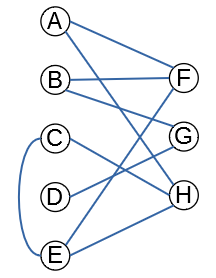
\includegraphics[width=2in]{final/sample-final-bipartite.png}}
\caption{\label{fig:clothing-dfs} Visualized Graph}
\end{figure}

\vspace{5pt}
{\bf (B)} The BST traversal of the graph is shown a




\vspace{20pt}
{\bf Question 5.}

\end{document}

